\section{Preliminary Results}
\label{sec:prelim}

본 실험에 앞서 구성 요소를 따로 시험했다(\cref{tab:prelim}). 이 절의 수치는 모두 주황색으로 표시한 임시 값이다. 파이프라인 관문 R1--R6과 측정원 시험(E-M4b-meas)의 수치도 여기에 모았다. 대부분은 \emph{파이프라인이 끝까지 동작하는지}를 본 소규모 시험이며, 논문의 결과나 방법의 근거로 쓰지 않는다. 표본이 작고, 과제가 하나(머그를 트레이에)이며, 일부는 시뮬 참값 좌표를 입력으로 썼기 때문이다.

\paragraph{공개 자료 분석.}
RoboDojo의 깨끗한 장면(standard)과 바뀐 장면(random) 점수를 공개 원자료로 계산했다(\cref{fig:prelim}). Astra는 \tentative{35.32에서 31.40으로 $-$11.1\%}, $\pi_{0.5}$는 20.92에서 5.82로 $-$72.2\%, Spatial Forcing은 $-$67.2\%, X-VLA는 $-$83.0\%였다(뒤 셋은 벤치마크 논문~\cite{robodojobench2026}의 표 3). 과제 재표집 부트스트랩으로 구한 Astra 하락의 95\% 구간은 \tentative{2.2--22.2\%}다. Astra만 과제 레시피 정보를 받았고, seed가 1개이며, 두 조건 모두 RGB를 직접 입력받아 인식 조건이 같지 않다. 따라서 이 분석은 동기일 뿐 결론이 아니다.

\begin{figure}[t]
\centering
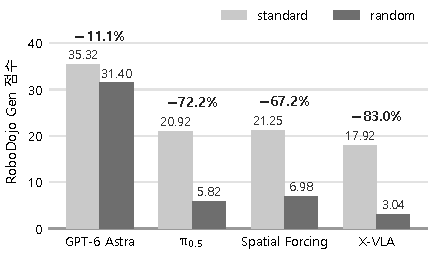
\includegraphics[width=\linewidth]{figures/prelim_drop.pdf}
\caption{\textbf{예비 분석.} RoboDojo Gen 12과제의 standard와 random 점수와 상대 하락. Astra 값은 RoboDojo Astra 평가~\cite{robodojo2026}의 공개 원자료로 우리가 계산했고(effort medium), $\pi_{0.5}$·Spatial Forcing·X-VLA 값은 벤치마크 논문~\cite{robodojobench2026}의 표 3이다. Astra 하락의 95\% 구간(과제 재표집)은 2.2--22.2\%이다. Astra만 레시피 정보를 받았고 seed가 1개이며 같은 인식 앞단 조건이 아니므로 예비 결과로만 본다.}
\label{fig:prelim}
\end{figure}


\paragraph{영점 선택기는 최빈 기준선보다 낮았다.}
학습하지 않은 Qwen3-VL을 typed 선택기로 쓴 사전 시험(DEV 30시드 $\times$ 섭동 3종, 스냅샷 2,387개 $\times$ 6질문)에서 4B의 정답률은 \tentative{0.483}, Gemma 4 E4B는 \tentative{0.425}로, 질문별 최빈 답 기준선 \tentative{0.669}보다 낮았다. 원인은 입력에 있었다. 당시 상태 텍스트는 술어의 참거짓만 싣고 그리퍼와 물체의 상대 위치가 없어, 방향·크기 질문에 답의 근거가 없었다. 로봇 기준 상대 위치 줄을 더하자 \tentative{+0.049} 올랐지만 최고 \tentative{0.532}로 여전히 기준선 아래였고, 모델은 대부분 한 보기로 쏠렸다(예: \texttt{dir\_z}는 100\% \texttt{down}). 그 상태 위에서 머리 카메라 이미지를 더한 이득은 \tentative{+0.0001}이었다. 이 결과로 학습하지 않은 선택기는 폐루프 실험에 쓰지 않고 기준선 행으로만 두며, 결정층은 학습을 거친 뒤 쓴다.

\paragraph{정답이 잘못 정의되어 있었다.}
같은 입력을 읽는 코드 규칙으로 옛 정답을 맞혀 보니 상한이 \texttt{dir\_xy} \tentative{0.920}, \texttt{dir\_z} \tentative{0.803}, \texttt{mag} \tentative{0.730}으로, 사전 등록한 관문(0.95)에 못 미쳤다. 옛 정답은 계획기의 명령 위치, 타이머, 스텝 안 단계 전환에 기대어 관측 상태로 결정되지 않는 양이었다. 그래서 \cref{sec:training}의 관측 정의 정답(labels\_v2)으로 바꾸었다. 1\,cm 단위 상태로는 관문에 못 미쳤고(\texttt{dir\_z} \tentative{0.856}), 1\,mm 단위 상태에서 \texttt{dir\_xy} \tentative{0.995}, \texttt{dir\_z} \tentative{0.991}, \texttt{mag} \tentative{0.988}로 통과했다. 모델 능력을 재기 전에 질문이 잘 정의되었는지를 먼저 확인해야 한다는 교훈을 사전 등록 절차에 넣었다.

\paragraph{학습 파이프라인 시험.}
결정층 SFT(단계 A)를 작은 풀(120편)에서 한 번 돌려, 데이터 생성, 라벨, 학습, LoRA 병합, vLLM 서빙, 평가가 끝까지 이어져 도는지 확인했다. 학습 때 줄이는 로그 확률과 추론 때 읽는 로그 확률이 같았고(작은 실제 구조 모델에서 상대 오차 \tentative{$10^{-4}$}), 병합한 모델을 서빙했을 때 동시 호출 4개 p95가 \tentative{0.307\,s}, 같은 입력의 답 뒤집힘이 \tentative{0/20}이었다. 정답률 수치는 인용하지 않는다. 입력 좌표가 시뮬 참값이고, 정답이 그 좌표에서 거의 기계적으로 나오며, 과제가 하나이고 무작위화가 없어 모델이 ``좌표를 읽는 법''을 배운 것 이상을 말해 주지 않기 때문이다. 융합 모델(단계 B)은 실제 4B 백본(BF16, LoRA r32)과 기본 크기 expert로 합성 40표본 50스텝 GPU 스모크를 했다. 결정 NLL은 \tentative{1.16에서 0.48}로 줄었고 flow matching 손실은 요동이 커 거의 줄지 않았으며, action expert에서 백본으로 가는 기울기 노름이 학습 전후 모두 \tentative{0.0}이었고(KI 차단 확인), 저장 뒤 다시 올린 모델의 예측 차가 \tentative{0.0}이었다. expert 한 번은 CUDA 그래프로 \tentative{23\,ms}, 문맥 순전파와 expert를 합친 한 번은 \tentative{120\,ms}였다. 공유 접두 트리 주의로 스냅샷당 순전파를 한 번으로 줄이자 옛 질문별 경로와 확률·기울기가 상대 오차 \tentative{$10^{-4}$} 안에서 같으면서 학습 처리량이 단계 A에서 \tentative{6.5배}, 단계 B에서 \tentative{약 8--12배} 올랐다. 실체크포인트 융합 폐루프(decide 한 순전파 + CUDA 그래프 chunk)는 Inspect Robots에서 오류 없이 돌았고, decide 지연은 시뮬레이터와 CPU를 나눠 쓴 조건에서 \tentative{255--376\,ms}였다.

\paragraph{폐루프와 평가 명령.}
M4를 켠 런타임이 Inspect Robots \texttt{eval()} 안에서 DEV 한 판을 끝까지 돌았다. 단계 A SFT 결정층 판은 \tentative{16.8\,s}에 성공했고(결정 호출 초당 \tentative{3.0}회, p95 \tentative{0.293\,s}, 실제 Astra 하트비트 2회), 영점 판은 같은 답을 반복하다 시간 초과로 실패했다. 이는 영점 선택기의 결과와 같은 모양이며 런타임 결함이 아니다. 같은 모의 판을 두 번 돌리면 실시간 배율이 달라도 행동 1,646개가 비트 단위로 같았다. E0.5 재생, RD, 보정, 폐루프 묶음이 각각 한 명령으로 끝까지 돌았다. 이 수치들은 한두 판의 파이프라인 확인이며 성공률이나 지연의 근거로 쓰지 않는다.

\paragraph{M4 (b)와 critic의 측정원 시험.}
융합 런타임에는 명시적 인식이 없으므로, (b)와 critic이 무엇을 측정으로 쓸지를 사전 등록 시험(E-M4b-meas)으로 골랐다. 실패 주입 5종과 무해 편차 3종을 넣은 DEV 270편에서, 단계 A 백본을 얼리고 학습한 확인 헤드 V1h의 세계 쪽 네 술어 평균 균형 정확도는 \tentative{0.949 [0.927, 0.965]}(ECE \tentative{0.004}, 커버리지 \tentative{0.905})였고, 명시적 인식 V0는 \tentative{0.596}, 영점 백본은 \tentative{0.750}이었다. 고유 감각 코드 규칙은 그리퍼 열림·쥠·쥔 채 들림을 \tentative{0.992--0.998}로 맞혀 하드 채널이 되었다. V1h에 관절 토크 충돌 규칙을 더하면 재현율이 \tentative{0.786}으로 V1h 단독 \tentative{0.871}보다 낮아 사전 등록 기준(0.80)에 못 미쳤고, 그래서 세계 쪽 경보를 V1h 단독으로 정했다. 헤드가 더하는 지연은 p95 \tentative{0.44\,ms}였다. 같은 장면·같은 정책 분포의 특권 라벨로 백본을 얼린 채 학습한 결과라, 본 데이터로 다시 잰다.

\paragraph{명시적 인식 기준선과 라벨.}
시뮬 기본 카메라에 SAM 3.1과 렌더러 깊이를 건 명시적 인식은 3D 중심 오차 중앙값이 \tentative{35\,mm}였고 손목 근거리에서 머그 검출을 \tentative{87.6\%} 놓쳤으며, 이 추정 좌표로 코드 규칙이 맞힌 정답률은 \tentative{0.612}로 최빈 \tentative{0.634}보다 낮았다. 이 결과가 인식을 런타임 의존에서 빼고 한 백본으로 융합한 근거 가운데 하나다. 스냅샷 풀 120편(스냅샷 1,200개, 분기 롤아웃 25,650회)의 결과 기반 라벨은 사전 등록 규칙이 고른 점수식이 거의 모든 보기를 최선으로 두어 판별력이 \tentative{0.006--0.069}에 그쳤으므로 거부권 용도로만 쓴다. 이때 재실행 복원이 1\,mm 기준을 넘은 행이 \tentative{410/6,627(6.2\%)} 나왔다. 조사 결과 같은 시드가 직전 실행 이력에 따라 몇 개의 이산 궤적 가운데 하나로 재생되었고(물리 엔진 장면 내부 상태로 추정), 이 행들은 무효로 빼며 다시 라벨하는 절차를 \tentative{준비 중}이다.

\paragraph{인식 앞단(모듈형 기준선).}
ROBOTIS 공개 데이터 두 과제(과제당 20편)의 머리 스테레오 영상에서 물체 3D 중심의 정지 구간 흔들림을 쟀다($f_x=367$\,px, 정답이 없으므로 흔들림의 상한으로 읽는다). GDINO + SAM 2.1과 SAM 3.1의 정지 흔들림 중앙값은 과제 1에서 \tentative{1.45와 1.42\,mm}, 과제 2에서 \tentative{2.41과 2.47\,mm}로 거의 같았고, p95는 \tentative{9--16\,mm}였다. 성패는 분할기가 아니라 검출 문구가 갈랐다. 과제 문장의 ``box''로는 흰 바구니를 \tentative{0/20}편, ``basket''으로는 \tentative{19/20}편 검출했다. 이 결과로 검출용 이름을 Astra가 장면을 보고 정하게 했다.

\paragraph{지연.}
\cref{fig:latency}는 각 층의 시간 예산을 모은 것이다. H200 한 장, 동시 호출 4개에서 4B 텍스트 + 머리 카메라 호출의 p95는 \tentative{0.261\,s}(반복 \tentative{0.265, 0.292\,s})였다. 이 값은 데이터를 본 뒤 워밍 절차를 고친 판이며, 처음 판은 \tentative{0.819\,s}였다. 모듈형 기준선의 vLLM 결정 호출에 머리 + 손목 두 장을 넣으면 모든 시퀀스를 한꺼번에 보내는 방식의 p95가 \tentative{0.29/0.53\,s}(두 판), 선행 시퀀스를 먼저 보내는 lead 방식이 \tentative{0.28/0.18\,s}였다. 캐시를 끄면 \tentative{0.63\,s}로 두 배가 되었다. 손목 이미지를 더해도 시각 토큰이 104개 늘 뿐이며, 병목은 토큰 수가 아니라 같은 이미지를 든 요청들의 동시 진입이었다. 배치 불변 모드를 켜면 고정 입력 20개의 답과 확률이 한 번도 바뀌지 않았다. Astra low의 첫 토큰은 \tentative{2.975\,s}(1회)였다.

\begin{figure}[t]
\centering
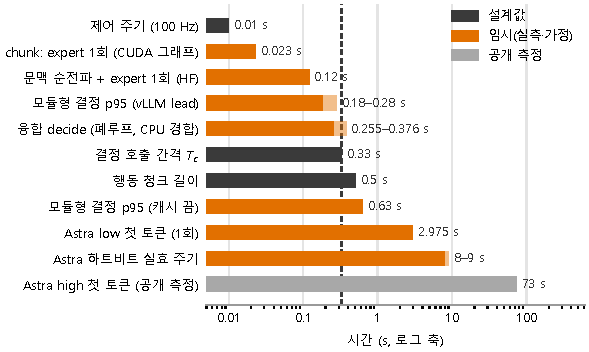
\includegraphics[width=\linewidth]{figures/latency_budget.pdf}
\caption{\textbf{층별 시간 예산(로그 축).} 검은 막대는 설계값, 주황 막대는 우리가 잰 임시 값 또는 가정값, 회색 막대는 공개 측정(Artificial Analysis, 2026-09-23, 우리가 잰 값 아님)이다. 모듈형 기준선의 vLLM 결정 호출(머리 + 손목, lead)은 호출 간격 $T_c=0.33$\,s 안에 들어온다. 융합 decide는 폐루프 파이프라인 시험에서 시뮬레이터와 CPU를 나눠 쓴 탓에 문턱을 넘기도 했고, chunk(expert, CUDA 그래프)는 수십 ms다. Astra는 그보다 한 자릿수 이상 느리므로 비동기로만 부른다. 주황 값은 모두 파이프라인 시험 값이다.}
\label{fig:latency}
\end{figure}


\paragraph{장면과 하네스.}
Inspect Robots v0.59.0은 Isaac Sim 5.1과 Isaac Lab 2.3 위에서 부팅되었고 세 시계 모드(sync, simlat, wall)가 모두 \tentative{16/16} 통과했으며, 하네스 오버헤드는 스텝당 \tentative{57--59\,$\mu$s}였다. random과 DR 변형을 구현한 뒤 특권 상태를 쓰는 오라클 계획기는 standard, random, DR에서 모두 \tentative{30/30}(P0)을 성공했다. 오라클은 시각 축의 영향을 받지 않으므로 이는 변형이 과제를 풀 수 없게 만들지 않았다는 확인일 뿐이다. 실시간 배율은 카메라를 끄면 \tentative{약 4.1}, 머리와 오른손목을 렌더하면 \tentative{약 1.18}이었다.

\begin{table*}[t]
\centering
\scriptsize
\setlength{\tabcolsep}{4pt}
\begin{tabular}{@{}p{0.14\linewidth}p{0.36\linewidth}p{0.44\linewidth}@{}}
\toprule
항목 & 조건 & 값 (모두 임시) \\
\midrule
영점 선택기 정답률 & DEV 2,387 스냅샷 $\times$ 6질문, 텍스트 + 머리 카메라 & \tentative{Qwen3-VL-4B 0.483, Gemma 4 E4B 0.425, 질문별 최빈 0.669} \\
상태 표현 진단 & 상대 위치 줄 추가, 이미지 추가 & \tentative{+0.049 [+0.043, +0.056], 최고 0.532 $<$ 0.669; 이미지 +0.0001 [$-$0.003, +0.004]} \\
정답 정의 관문 & 상태만 읽는 코드 규칙의 상한 & \tentative{옛 정답: dir\_xy 0.920, dir\_z 0.803, mag 0.730 (실패) / labels\_v2 1\,mm: 0.995, 0.991, 0.988 (통과)} \\
학습 파이프라인 & 단계 A SFT 1회(120편), 병합 BF16 서빙 & \tentative{학습 확률 = 추론 확률, p95 0.307\,s, 뒤집힘 0/20; 정답률은 인용 안 함} \\
융합 모델 스모크 & 실제 4B, GPU, 합성 40표본 50스텝 & \tentative{결정 NLL 1.16$\rightarrow$0.48, expert $\rightarrow$ 백본 기울기 0.0, 재적재 차 0.0; expert 23\,ms, 문맥+expert 120\,ms} \\
학습 처리량 & 공유 접두 트리 주의, H200 1장 & \tentative{옛 경로와 확률·기울기 차 rel $10^{-4}$ 이내; 단계 A 6.5배, 단계 B 약 8--12배} \\
폐루프 & Inspect Robots, DEV 1판, M4 C5 & \tentative{SFT 결정층 성공(16.8\,s, p95 0.293\,s), 영점 실패; 모의 판 행동 1,646개 비트 동일; 융합 decide 255--376\,ms} \\
(b)·critic 측정원 & E-M4b-meas, FI-DEV 270편 & \tentative{V1h 0.949 (V0 0.596, 영점 0.750); T1 0.992--0.998; V1h+토크 재현율 0.786 $<$ V1h 0.871; 헤드 +0.44\,ms} \\
명시적 인식 & SAM 3.1 + 렌더 깊이, R1-DEV & \tentative{3D 오차 중앙값 35\,mm, 손목 근거리 누락 87.6\%, 추정 좌표 정답률 0.612 $<$ 최빈 0.634} \\
결과 기반 라벨 & POOL 120편, 롤아웃 25,650 & \tentative{판별력 0.006--0.069 (거부권 용도); 복원 1\,mm 초과 6.2\% 행 무효} \\
결정 호출 지연 & H200, vLLM 0.30.0, 배치 불변, $N{=}4$, p95 & \tentative{머리만 0.261 (첫 판 0.819); 머리+손목 base 0.29/0.53, lead 0.28/0.18; 캐시 끔 0.63\,s} \\
Astra 지연 & effort low, 짧은 입력 1회 & \tentative{첫 토큰 2.975\,s} \\
인식 흔들림 & ROBOTIS 공개 데이터, 과제당 20편, $f_x{=}367$ & \tentative{정지 중앙값 1.42--2.47\,mm, p95 9--16\,mm; ``box'' 0/20, ``basket'' 19/20} \\
장면·하네스 & Inspect Robots, random5, 오라클 & \tentative{시계 3종 16/16, 오버헤드 57--59\,$\mu$s; 오라클 30/30 (std, random, DR); RTF 4.1(카메라 끔)/1.18(렌더)} \\
\bottomrule
\end{tabular}
\caption{\textbf{예비 결과 요약.} 모두 파이프라인 시험이거나 작은 표본의 사전 측정이며 본 결과가 아니다. 지연 값의 일부는 데이터를 본 뒤 절차를 바꾼 판이라 첫 판을 함께 적었다.}
\label{tab:prelim}
\end{table*}
